\section{Clustering}

\subsection{توضیحات کلی}

با استفاده از خوشه‌ سازی، سعی کردم دوربین‌ها را به دسته‌های مختلفی تقسیم کنم، و برای 
هر دسته مفهومی بیابم. نماینده‌ هر دوربین در این روش، یک بردار با اندازه‌ی 
$24 \times 7$
است، که در هر خانه‌ی آن تعداد تردد در آن ساعت از روزهفته قرار گرفته‌است. ۲۴ ساعت اول 
برابر با یک‌شنبه است، ۲۴ ساعت بعدی برای دو شنبه و الی آخر. پس بردار 
متناظر هر دوربین، تعداد تردد‌ها در هر ساعت از یک هفته را برای آن دوربین 
مشخص می‌کند. 

برای خوشه‌سازی از الگوریتم 
LDA یا 
\lr{Latent Dirichlet Allocation}
استفاده شده است، که همانطوری که در درس دیدیم استفاده اولیه آن پیدا کردن 
توزیع 
topic
های مختلف و کلمات آن‌ها برای هر مقاله است. با استفاده از این الگوریتم برای 
داده‌های تردد ماشین‌ها نیز می‌توانیم دقیقا به چنین توزیعی برسیم. 

یکی از متغییر‌های بسیار مهم در این بخش، 
\lr{cluster\underline{ }center}
است، که تعداد کلاستر‌های نهایی را مشخص می‌کند . با تغییر این متغییر این متغیر می‌توانیم تعابیر متفاوتی از داده‌ داشته باشیم. اما یکی از واضح‌ترین نتیجه‌‌ها برای
\mbox{\lr{cluster\underline{ }center = 3}}
به دست می‌آید که آن را در شکل‌های زیر می‌بینید: 

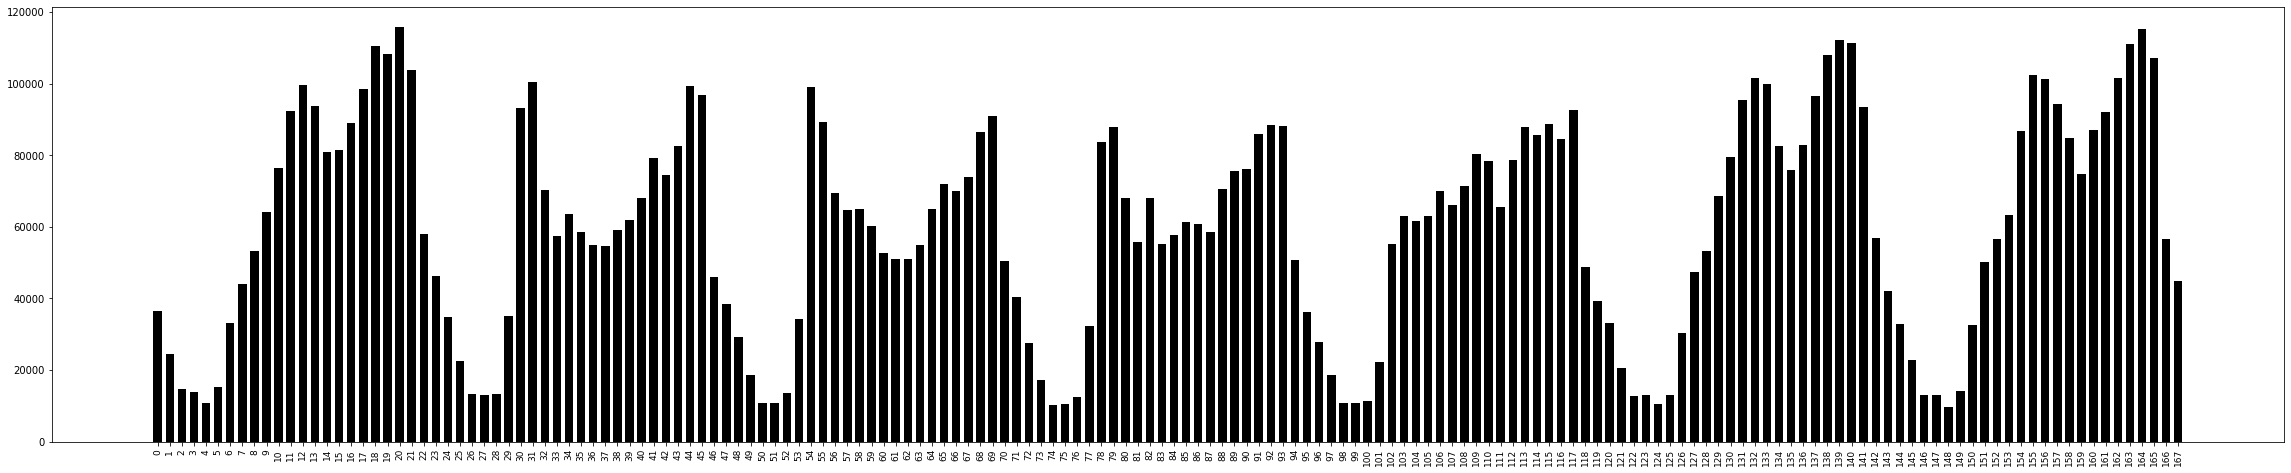
\includegraphics[scale=0.2]{images/Clustering/1.png}

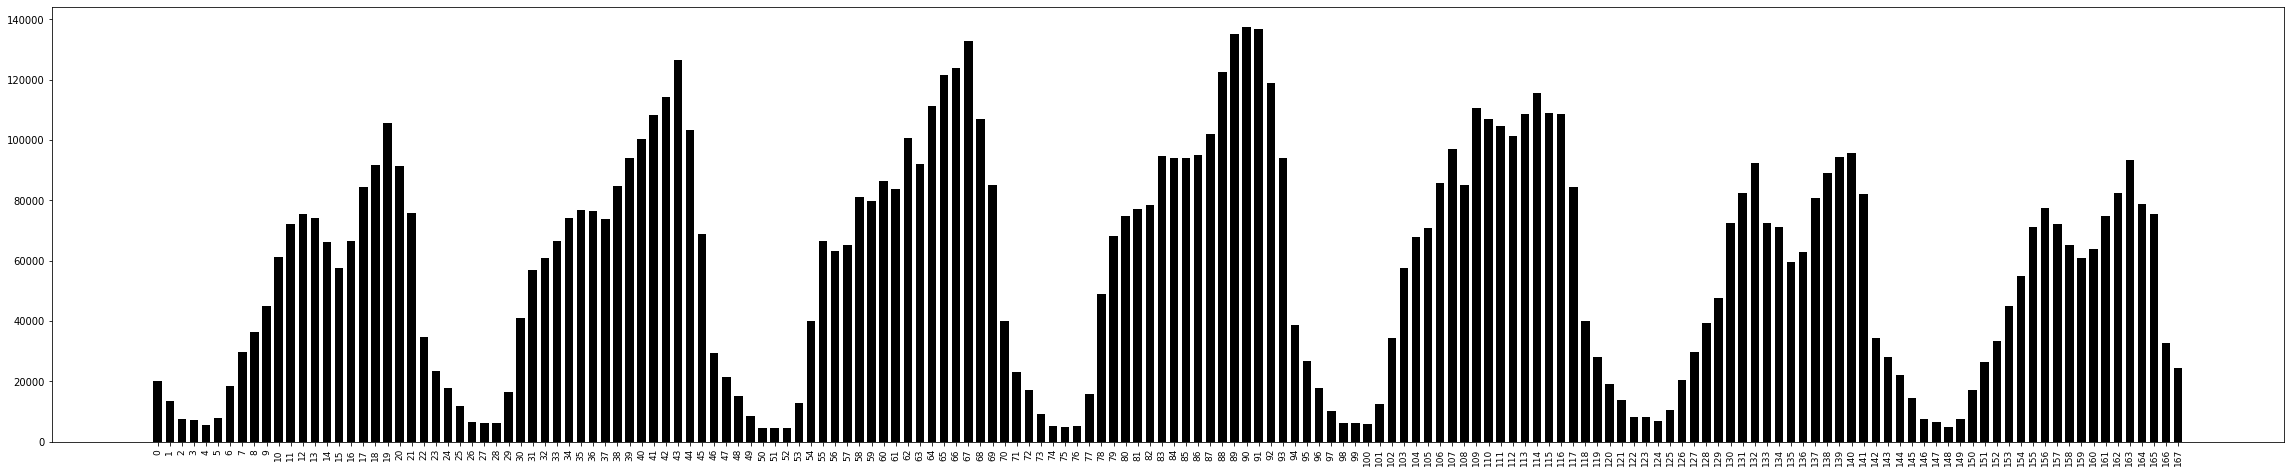
\includegraphics[scale=0.2]{images/Clustering/2.png}

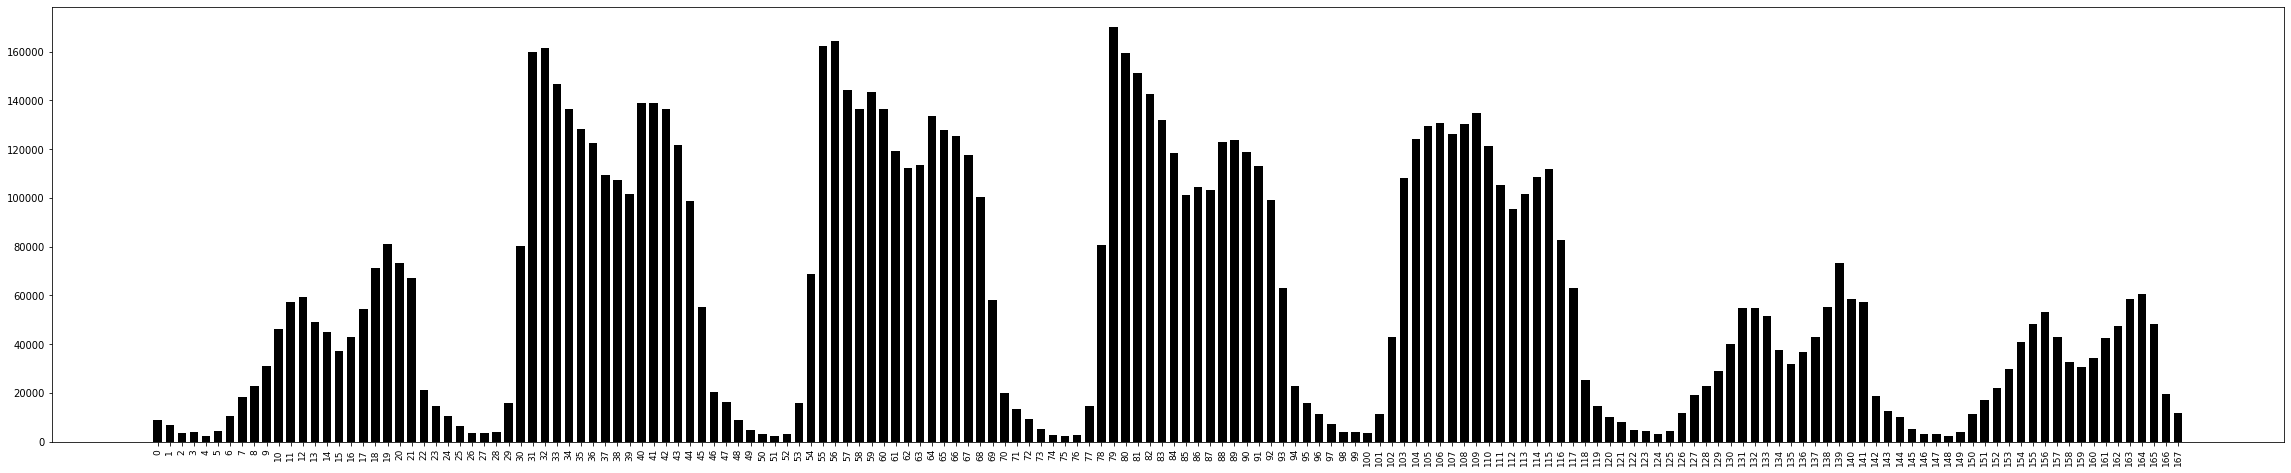
\includegraphics[scale=0.2]{images/Clustering/3.png}


\subsection{تحلیل نتایج}

مهم‌ترین نکته‌ی این سه تصویر، روند تغییر تردد‌ها در هر روز است. در دسته‌ی اول، 
تردد در ساعات اولیه روز افزایش می‌یابد، در هنگام ظهر کاهش پیدا می‌کند، سپس دوباره در 
شب افزایش پیدا می‌کند. در دسته‌ی دوم، تردد در صبح کم است، اما کم کم افزایش می‌یابد و در شب 
به اوج خود می‌رسد. دسته‌ی سوم روندی دقیقا عکس دسته‌ی دوم دارد، و بیشترین تردد را در صبح 
دارند و سپس کاهش می‌یابد. 

سه دسته‌ی بالا را می‌توانیم به این صورت تفسیر کنیم. دسته‌ی اول نقاط پر تردد شهر هستند، که هم در روز 
و هم در شب تردد بالایی دارند. این نقاط احتمال مکان‌هایی وسط شهر هستند که تمام 
طول روز تردد دارند ( البته طبیعتا تردد در ظهر کاهش می‌یابد). 
دسته‌ی دوم، احتمالا مکان‌های دیدنی و تفریحی و یا بازار‌های شبانه هستند 
که در طول روز تردد زیادی ندارند (به دلیل این که مردم مشغول کار و مدرسه و ... هستند). 
دسته‌ی سوم نیز احتمالا مکان‌هایی هستند که در طول روز تردد بالایی دارند، مانند مکان‌های اداری، مسیر مدارس و ادارات، یا دوربین‌های نزدیک به مثلا نانوایی‌ها. 

یک نکته‌ی بسیار جالب دیگری که در این تصاویر دیده می‌شود، این است که که تردد 
در روز‌های جمعه، شنبه و یک شنبه به طرز جالبی پایین است. با چک کردن این ۳ روز روی تقویم، فهمیدم که این روز‌ها 
تعطیل رسمی بوده‌اند (قیام ۱۵ خرداد و شهادت امام جعفر صادق (ع)). بسیار جالب است که این کاهش 
ترددها، فقط در دسته‌ی سوم رخ داده‌است، که دقیقا با شهود ما همخوانی دارد، که دسته‌ی سوم مکان‌هایی 
مانند مدارس و ادارات هستند. همچنین، الگوی کاهشی تردد در این سه روز از بین رفته‌ است 
که باز هم مطابق با الگوی پیدا شده است. 


این روش دسته‌بندی کردن دوربین‌ها می‌تواند فواید زیادی از جمله هدایت ترافیک، 
مکان درست بیلبوردهای  تبلیغاتی، مکان مناسب برای بعضی از فروشگاه‌های خاص و ... داشته باشد.